%%% Preamble
  \documentclass[11pt]{beamer}
  \usetheme{Boadilla}
  \useoutertheme{split}
  \useinnertheme{circles}
  \usepackage{fourier}
  \usefonttheme{structurebold}
  \usepackage{array}
  \usepackage[english]{babel}
  \usepackage{amsmath,amssymb}
  \usepackage[latin1]{inputenc}
  \usepackage{setspace}

  \usepackage{array}
  \usepackage{threeparttable}
  \usepackage{colortbl}
  \usepackage{multirow}
  \usepackage{amsthm}
  \usepackage{float,graphicx,color}
  \newtheorem*{thm}{Theorem}
  \theoremstyle{definition}
  \newtheorem*{defn}{Definition}
  \newcommand\boldline{\arrayrulewidth{1pt}\hline}
  \newcommand\ve{\varepsilon}
  \providecommand{\norm}[1]{\lVert#1\rVert}


  \setbeamercovered{dynamic}

  \title[Micro Engines]{Microfabrication of Little Engines}
  \author[Anderson and Lyon]{\textbf{Kyle Anderson} \and \textbf{Spencer Lyon}}
  \date{\today}

\begin{document}
\frame{\titlepage}


\section{Theory} \label{sec:theory}

  \subsection{Microfabrication} \label{sub:microfabrication}

    \begin{frame} \frametitle{Review Microfabrications}
    \begin{itemize}[<+->]
      \item During class we were exposed to microfabrication with carbon nano-tubes
      \item We designed small cantilevers and went through the fabrication process
      \item We then did took optical measurements to characterize the frequency response of the cantilevers
      \item With microfabrication there is potential for much more than just measuring resonant frequencies
    \end{itemize}
    \end{frame}

  \subsection{MEMS} \label{sub:mems}

    \begin{frame} \frametitle{MEMS Basics}
    \begin{itemize}[<+->]
      \item MEMS: micro-electromechanical systems.
      \item What are they used for?
      \begin{itemize}
        \item Wii remote accelerometer
        \item Inkjet printers
        \item Chemical detectors
        \item Motors
      \end{itemize}
      \item We wanted to make a motor
    \end{itemize}
    \end{frame}

\section{Design} \label{sec:design}

  \begin{frame} \frametitle{Our Goal}
      \begin{itemize}
        \item Our goal was to create and measure the thermo-induced displacement of a micro motor
      \end{itemize}
  \end{frame}

  \subsection{Optics} \label{sub:optics}

    \begin{frame}[t]\frametitle{Interferometer}
      \begin{itemize}
        \item To measure the displacement we thought we could use an interferometer
        \item We started with design from class and adapted it slightly:
      \end{itemize}
      \begin{figure}[ht]
          \centering
          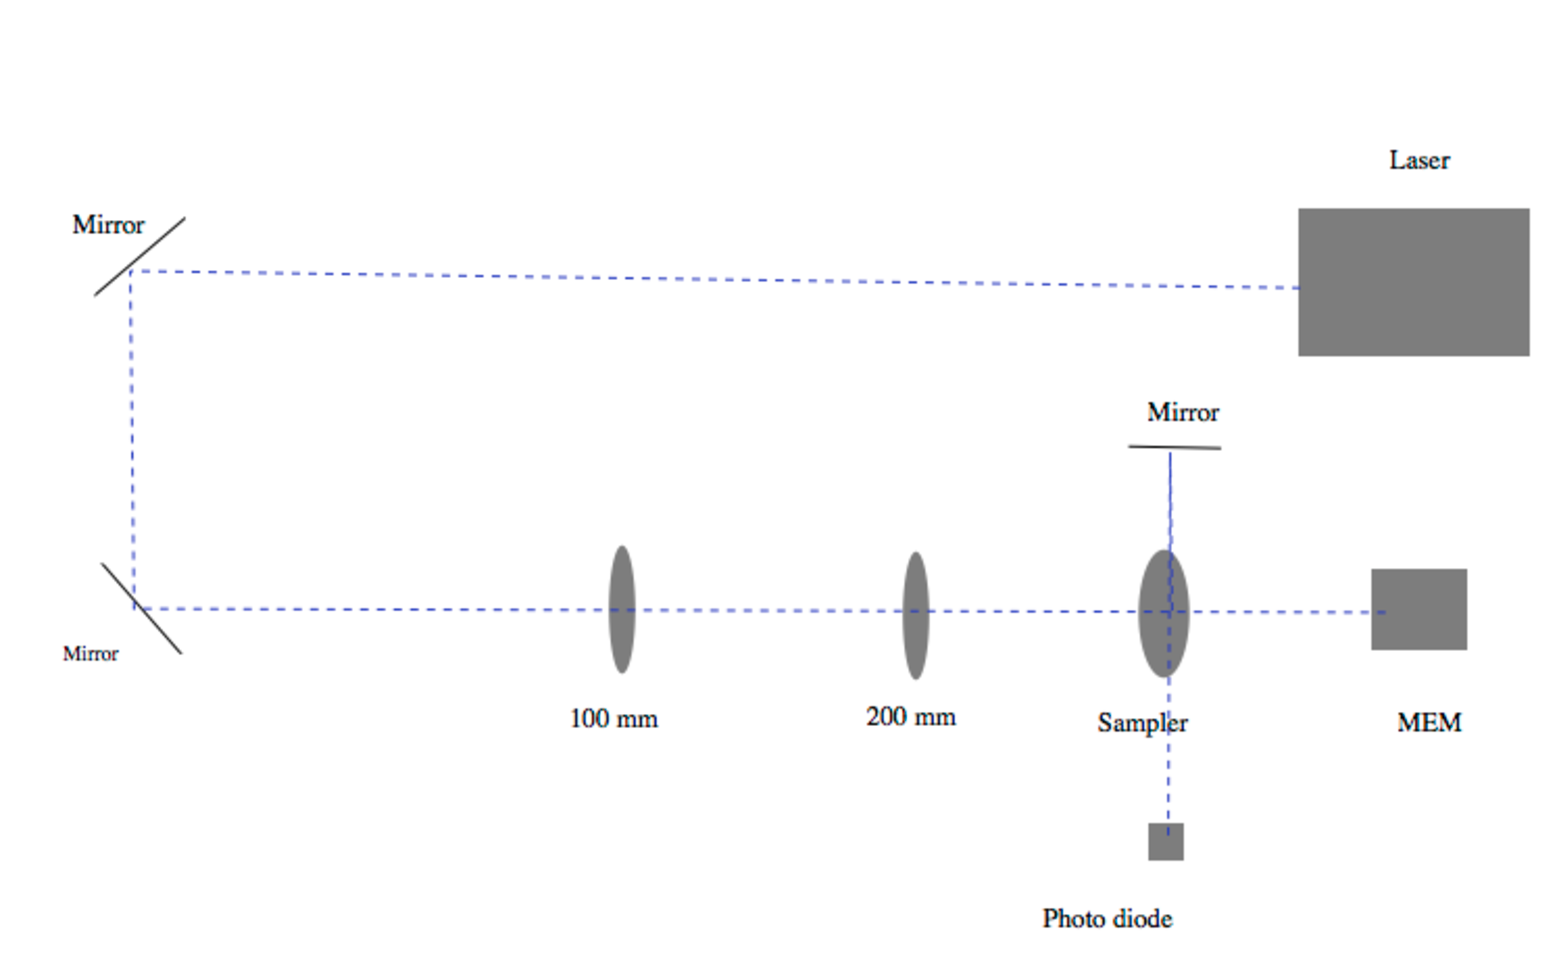
\includegraphics[width=4in, height=2in]{./Figures/InterferometerDesign.pdf}
          \label{fig:interferometer_design}
      \end{figure}
    \end{frame}

  \subsection{MEM} \label{sub:mem}

   \begin{frame} \frametitle{Our Motors Designs}
      \begin{columns}

      % Left Column
      \begin{column}{0.35 \textwidth}
      \begin{itemize}
        \item 4 designs:
        \begin{itemize}
          \item 2 straight legs
          \item 3 straight legs
          \item 2 angled legs
          \item 3 angled legs
        \end{itemize}
      \end{itemize}
    \end{column}

    % Right column
    \begin{column}{0.62\textwidth}
    \begin{figure}[ht]
          \centering
          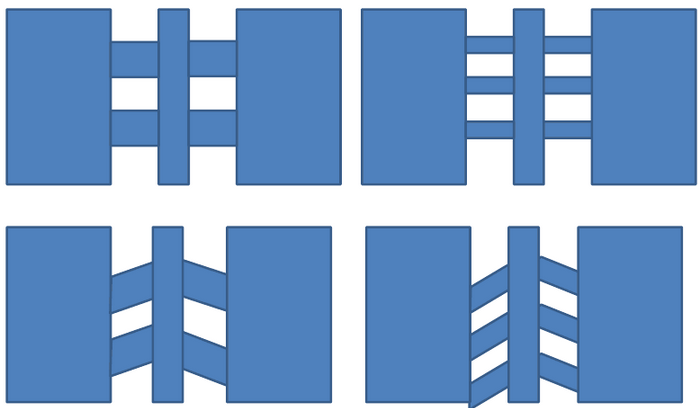
\includegraphics[width=2.6in, height=2.3in]{./Figures/EngineDesigns.png}
          \label{fig:sharpie}
      \end{figure}
    \end{column}
    \end{columns}
    \end{frame}

    \begin{frame}\frametitle{Mask from EE}
        \begin{figure}[ht]
          \centering
          \includegraphics[width=4in, height=2in]{./Figures/mask.jpg}
          \label{fig:mask}
      \end{figure}
    \end{frame}

\section{Procedure} \label{sec:procedure}

  \subsection{Fixing the Mask} \label{sub:fixing_the_mask}

    \begin{frame} [t]\frametitle{Sharpie!}
      \begin{itemize}[<+->]
        \item We needed to add the missing legs
        \item Bailey used a sharpie to draw them in
      \end{itemize}
    \end{frame}

    \begin{frame} [t]\frametitle{Sharpie!}
      \begin{itemize}
        \item We needed to add the missing legs
        \item Bailey used a sharpie to draw them in
      \end{itemize}
      \begin{figure}[ht]
          \centering
          \includegraphics[width=4in, height=2in]{./Figures/Sharpie.jpg}
          \label{fig:sharpie}
      \end{figure}
    \end{frame}

  \subsection{Deposition and Growth} \label{sub:deposition_and_growth}

    \begin{frame} \frametitle{Deposition}
      \begin{itemize}[<+->]
        \item We followed SOP to deposit iron (see picture and note sharpie marks)
      \end{itemize}
      \begin{figure}[ht]
          \centering
          \includegraphics[width=4in, height=2in]{./Figures/Deposition.jpg}
          \label{fig:deposition}
      \end{figure}
    \end{frame}

  \begin{frame} \frametitle{Growth}
      \begin{itemize}[<+->]
        \item Also followed SOP for growing carbon tubes (see image for infiltration details)
      \end{itemize}
      \begin{figure}[ht]
          \centering
          \includegraphics[width=4in, height=2in]{./Figures/Infiltration.jpg}
          \label{fig:infiltration}
      \end{figure}
    \end{frame}

  \subsection{Interferometer Setup} \label{sub:interferometer_setup}

    \begin{frame} \frametitle{Interferometer Setup}
      \begin{figure}[ht]
            \centering
            \includegraphics[width=4.3in, height=2.4in]{./Figures/Interferometer.jpg}
            \label{fig:interferometer_design}
        \end{figure}
    \end{frame}

\section{Setbacks} \label{sec:setbacks}

  \begin{frame} \frametitle{Precision}
    \begin{itemize}[<+->]
      \item Optical systems are difficult to set up
      \item We were trying to measure interference from very small surface ($<5mm$)
      \item We weren't able to get that working
      \item Bailed on the interferometer and went with simpler setup \dots
    \end{itemize}
  \end{frame}

  \begin{frame} \frametitle{Simple Optics}
      \begin{itemize}[<+->]
        \item Shine laser onto MEM, through lens, onto ruler 75cm away.
      \end{itemize}
      \begin{figure}[ht]
          \centering
          \includegraphics[width=3.7in, height=2.3in]{./Figures/SimpleOptics.jpg}
          \label{fig:sharpie}
      \end{figure}
    \end{frame}

  \begin{frame} \frametitle{Sampling Issues}
    \begin{itemize}[<+->]
      \item We made 4 different designs as outlined before
      \item When growing the tubes we could only have 4 in the furnace
      \item We forgot to do one of each design
      \item By chance we ended up with 3 of one design (3 angled legs) and 1 of another (2 angled legs)
    \end{itemize}
  \end{frame}

  \begin{frame} \frametitle{Fragile Motors}
    \begin{itemize}[<+->]
      \item They all ended up breaking before we could take meaningful data:
      \begin{enumerate}
        \item  One was lost
        \item One stuck to the wafer and broke when we tried to remove it
        \item One broke when we tried to move it
        \item One had a hole burned through it
      \end{enumerate}
    \end{itemize}
  \end{frame}

  \begin{frame} \frametitle{Broken Motor}
      \begin{figure}[ht]
          \centering
          \includegraphics[width=4in, height=2.6in]{./Figures/BrokenMotor.jpg}
          \label{fig:sharpie}
      \end{figure}
    \end{frame}

\section{Conclusion} \label{sec:conclusion}

  \begin{frame} \frametitle{Back to Drawing Board}
    \begin{itemize}[<+->]
      \item Applying voltage across motor induced heat
      \item However, we couldn't see any thermal expansion
      \item To fix this we could:
      \begin{itemize}
        \item Use a complete mask
        \item Make more samples (because some will break!)
        \item Thinner (fewer) legs = less resistance to expansion
        \item More controlled application of voltage
      \end{itemize}
    \end{itemize}
  \end{frame}

\end{document}
